
% used inside TikZ, thus must be accessible to PlasTeX as well
\usepackage[dvipsnames]{xcolor}

\newcommand*\cleartoleftpage{%
  \clearpage
  \ifodd\value{page}\thispagestyle{empty}\hbox{}\newpage\fi
}




\usepackage{tikz}
\usetikzlibrary{
	matrix,fit,shapes.callouts,shapes.arrows,shapes.misc,positioning,decorations.pathmorphing,arrows.meta,fpu,shapes.multipart,mindmap,arrows
}


% https://tex.stackexchange.com/a/72793
\tikzset{
	outlined arrow/.style args={#1 colored by #2 and #3}{		
		-latex,
		line width=#1,#2,
		postaction={draw,-latex,#3,line width=(#1)/3,shorten <=(#1)/4,shorten >=4.5*(#1)/3}
	}
}

%\tikzset{
%  disable rounded corners for decorations/.style={
%    /pgf/every decoration/.style={
%      /tikz/sharp corners
%    },
%  }
%}

\tikzset{>=latex}

\tikzset{
	% custom asymetric columnns
	left column/.style args={below #1}{at=(#1.south),anchor=north east,shift=({-.5em,-1em})},
	right column/.style args={below #1}{at=(#1.south),anchor=north west,shift=({.5em,-1em})},
	narrower left column/.style args={below #1}{at=(#1.south),anchor=north east,shift=({-.5em-.15\linewidth,-1em})},
	wider right column/.style args={below #1}{at=(#1.south),anchor=north west,shift=({.5em-.15\linewidth,-1em})},
	% custom styles
	thought/.style={dashed,rounded corners,font=\itshape},
	action/.style={solid,sharp corners},
	% FIXME: why not 2\pgfkeysvalueof ??
	wider sober/.style={
		fill=blue!10,align=justify,dotted,rectangle split,rectangle split parts=2,sharp corners,
		text width=.65*(\linewidth-1em)-1*\pgfkeysvalueof{/pgf/inner xsep}-2*\pgflinewidth
	},
	sober/.style={fill=blue!10,align=justify,dotted,rectangle split,rectangle split parts=2,sharp corners},
	mindful/.style={fill=blue!10,align=center,dotted},
	narrower autopilot/.style={
		fill=red!10,
		text width=.35*(\linewidth-1em)-1*\pgfkeysvalueof{/pgf/inner xsep}-2*\pgflinewidth
	},
	autopilot/.style={fill=red!10,dashed},
	sober arrow/.style={outlined arrow={.5mm colored by black and blue!40}},
	wide sober arrow/.style={outlined arrow={1mm colored by black and blue!40}},
	autopilot arrow/.style={outlined arrow={.5mm colored by black and red!40}},
	wide autopilot arrow/.style={outlined arrow={1mm colored by black and red!40}},
}

\def\soberName#1{\textbf{#1} \nodepart{two} }

\def\mbrpset#1{\pgfkeys{/mbrp/.cd,#1}}
\pgfkeys{/mbrp/.is family,/mbrp,
	title1/.initial=\undefined,
	title2/.initial=\undefined,
	autopilot/.store in=\mbrpAutopilot,
	brzda B/.initial={Zastavte se a vyskočte z autopilota.},
	brzda R/.store in=\mbrpBrzdaR,
	brzda R/.initial=\undefined,
	brzda Z/.initial={Několikrát se pomalu a pozorně nadýchěte a vydýchněte. Pozornost zaměřte na dech.},
	brzda D/.initial={Rozšiřte znovu svou pozornost na to, jak se cítíte. Nakolik to jde, zkuste to udělat s postojem otevřenosti a přijetí.},
	brzda A/.store in=\mbrpBrzdaA,
	brzda A/.initial=\undefined,
	%
	title/.initial=\undefined,
	title/.store in=\mbrpTitle,
	toc title/.initial=\relax,
	summary/.initial=\undefined,
	informal moments/.initial=\undefined,
	informal challenges/.initial=\undefined,
	informal activities/.initial=\undefined,
	% formal/.store in=\mbrpFormal,
	formal/.initial=\undefined
}


%\def\summaryAndPractices#1#2#3#4#5{
%}
%\def\recommendedPractices#1#2#3#4{
%}

\newcommand{\mbrpSession}[1]{
	\mbrpset{#1}
	\cleardoublepage
	\pgfkeysifdefined{/mbrp/toc title}%
		{\section[\pgfkeysvalueof{/mbrp/toc title}]{\mbrpTitle}}%
		{\section{\mbrpTitle}}
	\thispagestyle{start-session}

	\bgroup
		\begin{tcolorbox}[parbox=false,title=Shrnutí]
			{\let\item\par \par\pgfkeysvalueof{/mbrp/summary}\par}
		\end{tcolorbox}

		\clearpage

		\begin{tcolorbox}[title={Formální cvičení, plánovaná},parbox=false]
			Snažte se poslouchat nahrávky vedených cvičení všímavosti každý den či obden (4× až 6× za týden). Vyzkoušejte cvičit pokaždé ve stejnou dobu (např. před snídaní).

			Do dalšího sezení doporučujeme se zaměřit na cvičení:
				\begin{itemize*}
					\pgfkeysvalueof{/mbrp/formal}
				\end{itemize*}
			\medskip
			%\textbf{Neformální cvičení — za pochodu:}
			\tcbsubtitle{Neformální cvičení, za pochodu}
				\begin{description*}
					\item[Okamžiky:] \pgfkeysvalueof{/mbrp/informal moments}
					\item[Obtíže:] \pgfkeysvalueof{/mbrp/informal challenges}
					\item[Činnosti:] \pgfkeysvalueof{/mbrp/informal activities}
				\end{description*}
		\end{tcolorbox}
	\egroup
	\clearpage

	%\recommendedPractices{#2}{#3}{#4}{#5}
	%\summaryAndPractices%
	%	{\pgfkeysvalueof{/mbrp/summary}}%
	%	{\pgfkeysvalueof{/mbrp/formal}}%
	%	{\pgfkeysvalueof{/mbrp/informal moments}}%
	%	{\pgfkeysvalueof{/mbrp/informal challenges}}%
	%	{\pgfkeysvalueof{/mbrp/informal activities}}%
}


\newcommand{\soberSpace}[1]{
	\begin{adjustbox}{width=\linewidth,height=.9\textheight,keepaspectratio}
	\begin{tikzpicture}[
		every node/.style={
			align=center,
			text width=(\linewidth-1em)/2-2*\pgfkeysvalueof{/pgf/inner xsep}-2*\pgflinewidth,
			draw,
			rounded corners,
		},
		node distance=1em,
	]
	\mbrpset{#1}
	\node(top)[text width=.9\linewidth]{\textsc{\pgfkeysvalueof{/mbrp/title1}} \\ \pgfkeysvalueof{/mbrp/title2}};
	\node(a0)[narrower autopilot,draw=none,narrower left column=below top]{$\downarrow${} \textsc{Autopilot} $\downarrow$};
	\draw[autopilot arrow] (top)--(a0);
	\foreach [var=\type,var=\content,count=\curr,remember=\curr as \prev (initially 0)] in \mbrpAutopilot {
		\node(a\curr) [narrower autopilot,\type,below=of a\prev]{\content};
		\draw[autopilot arrow] (a\prev.south)--(a\curr.north);
	}


	\node(b1)[wider sober,wider right column=below top]{\soberName{Brzdi!} \pgfkeysvalueof{/mbrp/brzda B}};
	\node(b2)[wider sober,below=of b1]{\soberName{Roz-vhled!} Podívejte se bez posuzování na probíhající zkušenost: \begin{iitemize}\foreach\content in\mbrpBrzdaR{\item\content}\end{iitemize}};
	\node(b3)[wider sober,below=of b2]{\soberName{Zakotvi se!} \pgfkeysvalueof{/mbrp/brzda Z}};
	\node(b4)[wider sober,below=of b3]{\soberName{Doširoka se otevři!} \pgfkeysvalueof{/mbrp/brzda D}};
	\node(b5)[wider sober,below=of b4]{\soberName{Akce!} Jednejte z porozumění situaci, které máte. \begin{iitemize}\foreach\content in\mbrpBrzdaA{\item\content}\end{iitemize}};
	\begin{scope}
		\draw[sober arrow] (top) -- (b1);
		\draw[sober arrow] (b1) -- (b2);
		\draw[sober arrow] (b2) -- (b3);
		\draw[sober arrow] (b3) -- (b4);
		\draw[sober arrow] (b4) -- (b5);
	\end{scope}
	\end{tikzpicture}
	\end{adjustbox}
}

\newcommand{\soberSpaceEmpty}[1]{
	%\begin{adjustbox}{width=\linewidth,height=.85\textheight,keepaspectratio}
	\mbrpset{#1}
	\def\miniStrut{\rule[-.4ex]{0pt}{0pt}}
	\def\myslenkyPocityJednani{\leavevmode\lower.3ex\hbox{\vbox{\tiny\baselineskip=0pt\lineskip=-.3ex\hbox{myšlenky}\hbox{pocity}\hbox{jednání}}}}
	\def\teloPocityMysl{\leavevmode\lower.3ex\hbox{\vbox{\tiny\baselineskip=0pt\lineskip=-.3ex\hbox{tělo\miniStrut}\hbox{pocity\miniStrut}\hbox{mysl\miniStrut}}}}
	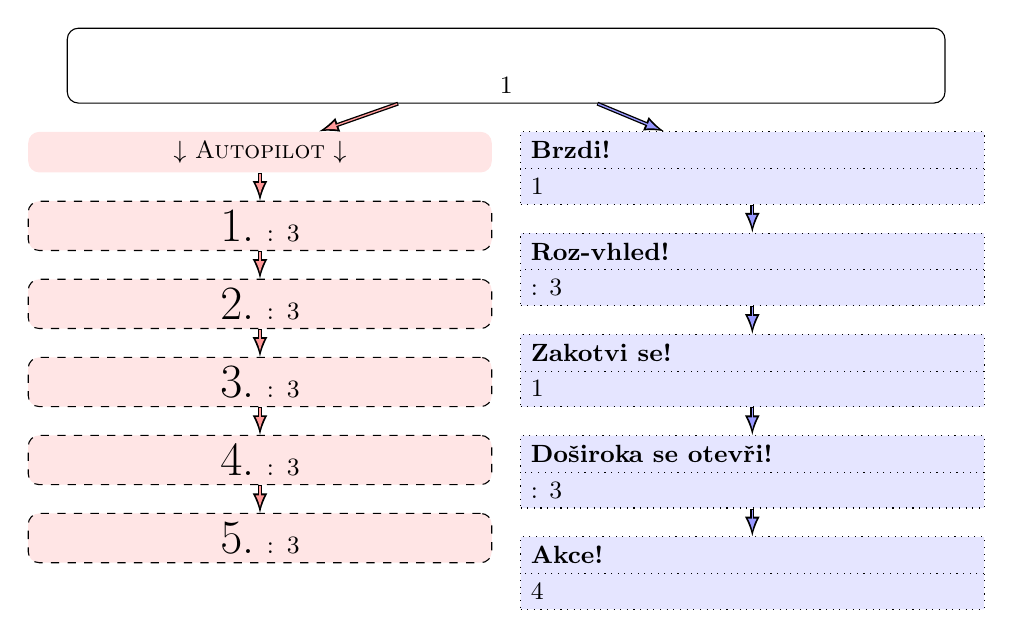
\begin{tikzpicture}[
		every node/.style={
			align=center,
			text width=(\linewidth-1em)/2-2*\pgfkeysvalueof{/pgf/inner xsep}-2*\pgflinewidth,
			minimum width=(\linewidth-1em)/2, %-2*\pgfkeysvalueof{/pgf/inner xsep}-2*\pgflinewidth,
			draw,
			rounded corners,
			font=\small
		},
		node distance=1em,
	]
	\node(top)[text width=.9\linewidth]{\textsc{\pgfkeysvalueof{/mbrp/title1}} \\ \rule{0em}{5ex}\Blank{1}};
	\node(a0)[autopilot,draw=none,left column=below top]{$\downarrow${} \textsc{Autopilot} $\downarrow$};
	\draw[autopilot arrow] (top)--(a0);
	\foreach [var=\curr,remember=\curr as \prev (initially 0)] in {1,2,3,4,5} {
		\node(a\curr) [autopilot,below=of a\prev]{{\LARGE \curr.} \myslenkyPocityJednani: \Blank{3}};
		\draw[autopilot arrow] (a\prev.south)--(a\curr.north);
	}


	\node(b1)[sober,right column=below top]{\soberName{Brzdi!} \Blank{1}};
	% \node(b2)[sober,below=of b1]{\soberName{Roz-vhled!} tělo\Blank{2}\linebreak pocity\Blank{2}\linebreak mysl\Blank{2}};
	\node(b2)[sober,below=of b1]{\soberName{Roz-vhled!} \teloPocityMysl: \Blank{3}};
	\node(b3)[sober,below=of b2]{\soberName{Zakotvi se!} \Blank{1}};
	%\node(b4)[sober,below=of b3]{\soberName{Doširoka se otevři!}  tělo\Blank{2}\linebreak pocity\Blank{2}\linebreak mysl\Blank{2}};
	\node(b4)[sober,below=of b3]{\soberName{Doširoka se otevři!} \teloPocityMysl: \Blank{3}};
	\node(b5)[sober,below=of b4]{\soberName{Akce!} \Blank{4}};

	\begin{scope}
		\draw[sober arrow] (top) -- (b1);
		\draw[sober arrow] (b1) -- (b2);
		\draw[sober arrow] (b2) -- (b3);
		\draw[sober arrow] (b3) -- (b4);
		\draw[sober arrow] (b4) -- (b5);
	\end{scope}
	\end{tikzpicture}
	%\end{adjustbox}
}

\def\pageBRZDAown#1#2#3{
	\clearpage\subsection{#1 \normalPencilLeftDown}
	\vskip-1em #2{} Co se pak stane, když fungujete na autopilota? Jak byste v takové situaci mohli použít \textsc{Brzd}u? Do každého kroku \textsc{Brzd}y vlastními slovy vepište, co byste udělali či vnímali.\par
	\vskip0pt minus1cm
	\soberSpaceEmpty{title1={#3}}
}



\def\pageGuesthouse{
	\clearpage
\subsection{Dům pro hosty}
	[\emph{Rúmí}; autor překladu neznámý]
	% FROM https://tex.stackexchange.com/a/196934/6758
	\newlength{\saveleftmargini}
	\setlength{\saveleftmargini}{\leftmargini}
	\setlength{\leftmargini}{0em}
	\begin{verse}
	Lidská bytost je jako dům pro hosty.\\
	Každé ráno přicházejí noví hosté.

	Radost, zármutek, podlost, \\
	okamžitý stav mysli přichází \\
	jako nečekaný host.

	Všechny přivítej a bav se s nimi! \\
	I když je to je houf starostí, \\
	které vtrhnou dovnitř a násilím rabují.

	I přesto přivítej každého hosta s úctou. \\
	Možná tě zbaví něčeho, \\
	co ti bránilo prožít nové radosti.

	Temné myšlenky, stud a zlobu \\
	přivítej s úsměvem u dveří \\
	a pozvi je dál.

	Za každého, kdo přijde, buď vděčný, \\
	protože ti jej osud posílá \\
	jako učitele.
	\end{verse}
	\setlength{\leftmargini}{\saveleftmargini}
	\vfill
}


\def\pageBRZDA{
	\clearpage
	\subsection{\textsc{Brzda}}
		\emph{\textsc{Brzda} je cvičení všímavosti „za pochodu“, které můžete použít kdekoliv a kdykoliv, protože je krátké, jednoduché a přizpůsobivé.} Můžete ho udělat za pár sekund i mu dát několik minut. Lze ho použít ve stresující situaci, když jste rozčilení či zakoušíte nutkání či vnitřní impulsy k jednání, kterému se chcete vyhnout. Je užitečné, i když jde všechno hladce, cítíte se dobře, či kdykoliv chcete být duchem „více tady“ k ocenění odehrávající se přítomnosti. Může vám pomoci k vyskočení z reaktivního autopilota a být si víc vědomý v tom, jak v nastalé situaci budete jednat.


		\begin{itemize}
		\itemStop{B}{Brzdi.} Šlápněte na brzdu a zastavte se, abyste toto cvičení mohli udělat. Je to první krok, kterým vystoupíte z autopilota.
		\itemStop{R}{Roz-vhled.} Rozhlédněte se uvnitř sebe, ve své svou momentální zkušenosti, a rozeberte ji na části: tělesné počitky, pocity, myšlenky. Zkuste se na ně podívat s určitou zvědavostí a bez odsuzování.
		\itemStop{Z}{Zakotvi se.} Udělejte několik pomalých nádechů a výdechů a zakotvěte přitom svou pozornost v tělesných počitcích, které dýchání doprovázejí.
		\itemStop{D\kern-.1em}{Doširoka se otevři.} Rozšiřte pozornost od dechu na celé tělo a pak i na celou situaci, ve které se nacházíte.
		\itemStop{A}{Akce.} Jednete v nastalé situaci s vnitřní orientací, nenechte jen proběhnout automatickou reakci. Buďte aktivní, ne reaktivní. Uvědomte si, že ve svém jednání máte na výběr. Zamyslete se nad tím, co v tuto chvíli potřebujete a jak byste se o sebe nejlépe postarali.
		\end{itemize}
	}


	\def\pagePracticeLog{
		\par\vfill\pagebreak % this will acutally flush the previous page (unlike clearpage) and \newgeometry won't affect the previous page
		\cleartoleftpage
		\newgeometry{left=1cm,right=1cm,top=1cm,bottom=1cm}
		\thispagestyle{empty}
		\bgroup
		\subsection{Záznam cvičení \normalPencilLeftDown}
			\ifplastex
				\def\myStrut{...}
				\begin{tabular}{l|l|l|l}
					% PASTED TWICE
					{datum \\ den } & pravidelné cvičení & cvičení za pochodu & { poznámky \\ postřehy  } \\
					& Vyhraďte si čas na nahrávku & {
						\textbf{všímavé zastavení}: náhodná chvíle k napojení na sebe \\
						\textbf{všímavé zvládání obtíží}: \textsc{Brzda} v náročné situaci \\
						\textbf{všímavé činnosti}: jídlo, chůze, domácí práce, pohyb venku } & \\
					& {Co jsem cvičil? \\  Jak dlouho?} & {Co jsem dělal? \\ Kolikrát? } & \\
					\hline \myStrut & \myStrut & \myStrut & \myStrut \\
					\hline \myStrut & \myStrut & \myStrut & \myStrut \\
					\hline \myStrut & \myStrut & \myStrut & \myStrut \\
					\hline \myStrut & \myStrut & \myStrut & \myStrut \\
					\hline \myStrut & \myStrut & \myStrut & \myStrut \\
					\hline \myStrut & \myStrut & \myStrut & \myStrut \\
					\hline \myStrut & \myStrut & \myStrut & \myStrut \\
				\end{tabular}
			\else
				\def\myStrut{\rule{0pt}{\dimexpr(\pagewidth-8em-2cm-6em)/7}} % {.07\textheight}}
				\footnotesize
				\begin{adjustbox}{angle=90}
				\begin{tblr}{
					width=.92\textheight,
					colspec={X[l,1.3]|X[l,4]|X[l,4]|X[l,2]},
					%row{2}={font=\tiny}
				}
					% PASTED TWICE
					%{datum \\ den } & pravidelné cvičení & cvičení za pochodu & { poznámky \\ postřehy  } \\
					%& Vyhraďte si čas na nahrávku & {
					%	\textbf{všímavé zastavení}: náhodná chvíle k napojení na sebe \\
					%	\textbf{všímavé zvládání obtíží}: \textsc{Brzda} v náročné situaci \\
					%	\textbf{všímavé činnosti}: jídlo, chůze, domácí práce, pohyb venku } & \\
					%& {Co jsem cvičil? \\  Jak dlouho?} & {Co jsem dělal? \\ Kolikrát? } & \\
					{datum \\ den } & {
						\textbf{pravidelné cvičení} \\
						{\tiny čas vyhrazený na nahrávku} \\
						Co jsem cvičil? Jak dlouho?
					} & {
						\textbf{cvičení za pochodu}  \\
						\textbf{okamžiky}: náhodné napojení na sebe \\
						\textbf{obtíže}: \textsc{Brzda} v náročné situaci \\
						\textbf{činnosti}: jídlo, chůze, domácí práce, pohyb venku \\
						Co jsem dělal? Kolikrát?
					} & { poznámky \\ postřehy  } \\
					\hline \myStrut & \myStrut & \myStrut & \myStrut \\
					\hline \myStrut & \myStrut & \myStrut & \myStrut \\
					\hline \myStrut & \myStrut & \myStrut & \myStrut \\
					\hline \myStrut & \myStrut & \myStrut & \myStrut \\
					\hline \myStrut & \myStrut & \myStrut & \myStrut \\
					\hline \myStrut & \myStrut & \myStrut & \myStrut \\
					\hline \myStrut & \myStrut & \myStrut & \myStrut \\
				\end{tblr}
				\end{adjustbox}
			\fi
		\egroup
		\restoregeometry
	}


